%+TITLE: Introducción
%+DESCRIPTION: Introducción y objetivo del curso
\documentclass[11pt,a4paper]{article}

\usepackage[utf8]{inputenc}
\usepackage[T1]{fontenc}
\usepackage[spanish,es-nodecimaldot]{babel}
\usepackage{lmodern}
\usepackage{amsmath,amssymb,mathtools}
\usepackage{graphicx}
\usepackage{xcolor}
\usepackage{geometry}
\usepackage{enumitem}
\usepackage{microtype}

\geometry{margin=2.3cm}
\setlength{\parindent}{0pt}
\setlength{\parskip}{0.65em}
\setlist[itemize]{leftmargin=1.6em,itemsep=0.25em,topsep=0.25em}

\definecolor{title-red}{RGB}{165,25,20}
\definecolor{concept-green}{RGB}{20,125,45}
\newcommand{\concept}[1]{\textcolor{concept-green}{#1}}

\newcommand{\ket}[1]{\left|#1\right\rangle}
\newcommand{\bra}[1]{\left\langle#1\right|}
\newcommand{\braket}[2]{\left\langle #1\middle|#2\right\rangle}
\newcommand{\hc}{\mathrm{h.c.}}
\newcommand{\Tr}{\operatorname{Tr}}
\newcommand{\Diffs}{\mathrm{Diffs}}

\begin{document}

Este curso se ocupa de física fundamental. Es decir, va en la línea de preguntarse por las leyes fundamentales de la naturaleza. Nuestra descripción fundamental de la naturaleza, hasta donde han podido confirmar los experimentos, se basa en la teoría cuántica de campos (QFT) y la relatividad general (GR).

\begin{align*}
  \text{Mecánica cuántica}
  +\text{ relatividad especial}
  +\text{ campos clásicos}
  &\longrightarrow \text{QFT},\\
  \text{Relatividad especial}
  +\text{ campos clásicos}
  +\text{ espacios curvos}
  &\longrightarrow \text{GR}.
\end{align*}

Este es el marco teórico, el escenario. Los actores son los campos (partículas) fundamentales.

\begin{center}
  \begin{figure}
  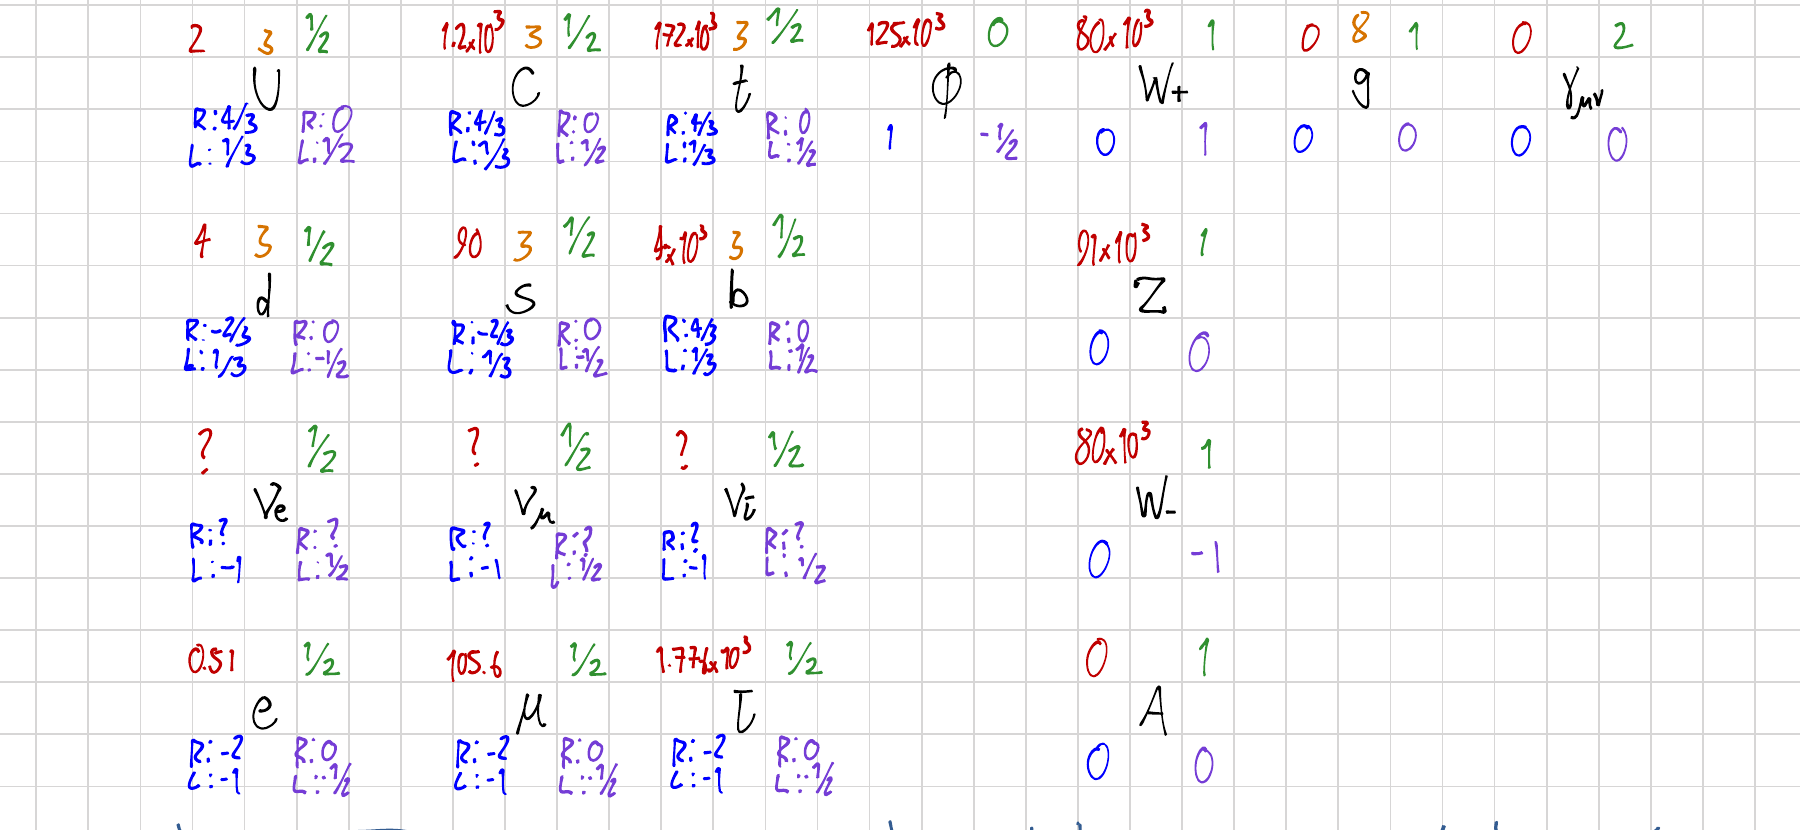
\includegraphics[width=\textwidth]{figures/tabla_modelo_estandar.png}

  \caption{Tabla manuscrita de campos y números cuánticos. En rojo la masa en $\mathrm{MeV}/c^2$, en verde el espín, en azul la hipercarga, en violeta el isospín, y en naranja la representación de color (singlete cuando no se indica).}
  \end{figure}
\end{center}

La acción que describe esta teoría (resume todo lo que sabemos sobre la naturaleza) es

{\small
\begin{align*}
S=\int d^4x\,\sqrt{-g}\Bigg(&
 \frac{1}{2}M_{\mathrm P}^{2}R
 -M_{\mathrm{Pl}}^{2}\Lambda
 -\frac{1}{4}F_{\mu\nu}F^{\mu\nu}
 +i\bar\psi\,\not D\psi+\hc
 +\bar\psi_iY_{ij}\psi_j\phi+\hc\\
&-\lvert D_\mu\phi\rvert^2
 -V(\phi)
 +\theta F_{\mu\nu}\widetilde F^{\mu\nu}
 +(\text{materia oscura, inflación, masa de los }\nu\text{'s})
\Bigg).
\end{align*}
}

Crucial en esta descripción es la simetría
\[
  SU(3)\times SU_L(2)\times U(1)\times \Diffs.
\]

Al final escribí los términos que sabemos que faltan porque hay experimentos que nos lo indican.

El propósito de este curso es entender lo que quiere decir todo esto a nivel clásico. Para hacer cálculos que podamos comparar con el experimento, necesitamos la mecánica cuántica y las técnicas de QFT.

\end{document}
